% press command+option+B to build, or change "Auto Build: Run" in Settings.

% \documentclass[12pt]{book}
\documentclass{book}

\usepackage{xeCJK}
\usepackage{geometry}
\usepackage{titlesec}
\usepackage{bm}
\usepackage{underlin}
\usepackage{wrapfig}
\usepackage{caption}
\usepackage{graphicx}
\usepackage{pdfpages}
\usepackage{multirow}%表格合并行列单元格

% 分栏并浮动图片
\usepackage{float}
\usepackage{multicol}
\usepackage[none]{hyphenat}
\usepackage{appendix}

% 数学
\usepackage{unicode-math}%正体希腊字母
\usepackage{mathrsfs}
\usepackage{amsfonts}

% 设置图书版式
\usepackage{marginnote}%侧栏
\usepackage{fancyhdr}%页眉页脚页码
\usepackage{indentfirst}%首段空两格
\usepackage{mdframed}%加阴影
\usepackage{color}%特殊字体颜色
\usepackage{setspace}%行距

\usepackage{hyperref}%所有网页用超链接同步挂靠

%行号
\usepackage{lineno}

\def\<{\hspace{0em}<\hspace{0em}}

\def\>{\hspace{0em}>\hspace{0em}}

\def\wz#1{%网址
    % \href{#1}{\texttt{#1}}
    \texttt{#1}
}

\def\jz#1{%原书脚注
    \footnote{#1}
}

\def\yz#1{%译注
    \footnote{\textsl{译注:}#1}
}

\def\dm#1{%代码
    {\xeCJKsetup{CJKecglue={\hskip 0em}}
    \hspace{0em}\texttt{#1}}\hspace{0em}}

\def\dmh#1{%代码行
    {\xeCJKsetup{CJKecglue={\hskip 0pt}}
    >> \texttt{#1}}
}

\def\celan#1{%侧栏TODO三角形方向
$\blacktriangleright$
\marginpar{
        $\blacktriangleleft$\textsf{#1}
    }
}

\newenvironment{exclamation}[1][!]%原书的圆圈感叹号
{
    \begin{mdframed}
        \textcircled{#1} \quad
        \sffamily
}{      
    \rmfamily
    \end{mdframed}
}

\newenvironment{dmd}{%代码段
    \xeCJKsetup{CJKecglue={\hskip 0pt}}
    \ttfamily
    \setlength{\parindent}{0pt}
}{
    \rmfamily
}

%代码清单,暂时定两个,之后再统一
\newenvironment{codelist}[2][TODO代码清单序号]{
    \begin{mdframed}
        \setlength{\parindent}{0pt}
        \textbf{清单 #1}

        \textbf{——效果——}

        #2 
    
        \textbf{——源码——} 
        % 用verbatim的时候这里会有一个奇怪的空行TODO
        % \begin{dmd}
            
}{
        % \end{dmd}
    \end{mdframed}
}

%字体
\setCJKmainfont[
    BoldFont={NotoSerifCJKsc-Bold},
    ItalicFont={Kai},
    SlantedFont={STFangsong}]
    {STSongti-SC-Regular}
\setCJKsansfont[
    ItalicFont={SmileySans-Oblique},
    SlantedFont={STFangsong}]
    {NotoSansCJKsc-DemiLight}
\setCJKmonofont[
    % ItalicFont={SmileySans-Oblique},
    SlantedFont={STFangsong}]
    {STYuanti-SC-Regular}
\setmonofont[
    ItalicFont={LMMono10-Italic},
    SlantedFont={SFMono-RegularItalic}
    ]
    {LMMono10-Regular}



\title{关于\LaTeX 的那些你想知道却从不敢问的问题\\{\small 或者说,如何在不会使用\LaTeX 的情况下使用\LaTeX }\\~\\Tout ce que vous avez toujours voulu savoir sur \LaTeX \ sans jamais oser le demander\\{\small Ou comment utiliser \LaTeX \ quand on n'y connaît goutte}\\~\\ ver. 1.5}
\author{Vincent Lozano 著}

\begin{document}
\maketitle
\tableofcontents
\mainmatter

%正文版式
\newgeometry{
    % inner = 2cm, outer = 4cm,
    % top = 2.5cm, bottom=2.5cm, 
    marginparwidth = 2cm, marginparsep = 0.5cm,
    % includeheadfoot
}
\pagestyle{fancy}
\fancyhead{} 
\fancyhead[RO,LE]{\thepage}
\fancyfoot{}
% \setlength{\headheight}{30pt}
% \renewcommand{\headrulewidth}{0.4pt}
% \renewcommand{\footrulewidth}{0pt}
% \setlength{\headwidth}{\linewidth + \marginparwidth + \marginparsep}
\setlength{\parskip}{3pt}
\setstretch{1.1}%倍行距

\chapter*{序}

\begin{epigraphe}{《便西拉智训》42:14}
    男人的邪恶\\胜过女人的善良\jz{
    本书的章首引言来自《旧约》与《新约》,将它们引用在这里纯粹是我一手挑动的——有时,这些句子中带有一些与章标题相关的内容(\textsl{译注}:本译文保留宗教相关内容,不代表译者对任何宗教文献中任何语句的认可或否定。本书未标注“\textsl{译注}”字样的脚注均为原书脚注)。}。\yz{本书将《便西拉智训》(天主教译为《德训篇》)作为《圣经》的一部分,但其实为《诗歌智慧书》的一部分,似乎属于次经,即在一些教派中不被承认作为《圣经》的一部分出现。}
\end{epigraphe}

\section*{从前……}

一切始于1990年年初。我当时正在PC 286计算机上使用称为\emph{WordPerfect}的软件,以此入门人们所谓的“文字处理”。这款软件现在仍然存在,并且由Corel公司维护,运行在日后拥有响当当名头的MS-DOS中。MS-DOS集成了用以粗略预览文档的接口,尤其允许用户“看到代码”,也就是借助一种标记语言将文档可视化,以灵活地控制。

稍晚些时间,随着Windows 3.1迅速风靡,人们突如其来地追求图形界面,我虽然仍情有不甘,却逐渐说服了自己去使用那款在今天很出名的文字处理软件——的2.0版(后面还带个小小的字母,在当时那可真是重大的升级)……但我日后才知道,这个版本有个很有趣的“特性”:文件体积过大,超过了某个特定的值时,会出现保存失败的情况!这时,你既不能保存,也不能恢复文档。有些头铁的朋友尝试先删除几行再保存,但这种撞大运的解决方案并没能成功……

当时,大家毫不掩饰地嘲讽这些“你懂的”公司制作的软件\jz{
    这些被嘲讽的对象中,我们可以看到一些名场面:通用汽车公司老板对比尔·盖茨挑衅性言论的回应(\textsl{译注}:可能是指比尔·盖茨的观点,即如果汽车工业能够像计算机领域一样发展,那么一辆汽车只需要25美元就能买到,并且消耗1加仑汽油就能跑1000英里。作为回应,通用汽车方面罗列了一系列言论来嘲讽,例如“如果那样,那么想要汽车熄火,需要点击开始菜单”),以及罗伯托·迪·科斯莫(Roberto Di Cosmo)的“赛博空间中的陷阱”(piège dans le cyberespace)。
}——这里就不点名了。我周围的大多数人躺平地选择了接受,认为使用这些堂而皇之不给出警告的可悲的跟风之流是正常现象。软件的这种“特性”坚定了我的信念:\emph{我绝不使用这种软件}。当时还在攻读工程师学位的我意识到,我今后的部分工作将会集中在起草文档和使用通用的信息系统上。为此,我需要足够健壮的工具。

我是在让·莫奈大学(Université Jean Monnet)和圣-埃蒂安高等矿业学校(École des Mines de Saint-Étienne)攻读DEA(现在叫master recherche)\yz{
    DEA即diplôme d'études approfondies,法国教育体系下的一种学位。
}时相继接触UNIX和Linux的。那时(1993~1994年),在我刚写论文的开头时,“拉泰克”(latèque)这个词就开始围着我转。这里问题似乎是要找到一款能排出数学公式的软件,而说到撰写理科文档,\LaTeX 似乎显然是避不开的\emph{唯一}答案。说实话,找软件这种问题甚至都根本没出现过!

于是,我着手把这个叫做\LaTeX 的“玩意儿”装在Mac系统(安装的发行版叫Oz\TeX )和另一个由古登堡(Gutenberg)协会支持的发行版系统——Solaris上。为此,我还得去收买一个系统管理员,让他同意创建一个特权用户\texttt{texadm},用来管理那个发行版……

1994年年初,我带着坚定的意志使用\LaTeX 开始写论文。在1995年,在被我发现的种种技巧激起的兴趣的巨大感召下,% 此句翻译不好:enthou- siasmé par ce que je découvrais, TODO
我着手为同事和实验室起草用于入门\LaTeX 的指导手册。这个手册就是本书的原型。在1997年,在练习了两年并一只脚踏入了排版领域后,我更坚定了自己的看法:\LaTeX 绝对是写严肃文件的首选软件:它有对版面(mise en page)的全面控制,有对参考文献的管理,支持索引(通用名称和作者名),能轻松操作文件。最重要的是,\emph{排版的结果很好看}。从那时起,这就是支撑我使用\LaTeX 的最强大而无可争辩的理由。

今天,作为国立圣-埃蒂安工程师学院(École Nationale d’ingénieurs de Saint-Étienne)的计算机高级讲师,我用\LaTeX 来起草理科文档和教学材料。几年使用下来,我仍然在学习和发现,也仍然会对项目贡献者提出的各种扩展啧啧称奇。这些扩展使\LaTeX 成为了充满宝藏的巴扎(bazar),成为了一款名副其实地朝着更高工效发展的\jz{
    并不是指那些诸如在菜单中添加一个功能入口、在弹出对话框时添加个提示音的“提效”。
}、始终以“产出优美的工作成果”为目标的卓越而独特的工具。

\section*{本书结构}

本书是针对“使用\LaTeX 进行文字处理”的介绍。它不是一本参考手册,但本书的写作目标是传授读者使用\LaTeX 的基本知识,并在可能情况下,让读者对它感兴趣。读者可以在本书中找到\emph{开始}使用\LaTeX 的必要信息和起草文档的建议。为了提升阅读体验,我们“高明地”将本书分为了若干章节,并配有附录。
本书首先介绍\LaTeX 的基础知识:
\begin{description}

\item[基本原则]展示\LaTeX 的基本原理。为了读懂本书的剩余部分,需要阅读本章。

\item[需要了解的知识]展示标准工具。为了起草一篇简单的文档,需要了解这些知识。

\item[数学排版]如何生成数学式。

\item[成为小魔仙]慢慢深入\LaTeX 的各组件。适合想要以让人满意的方式使用\LaTeX 的人阅读。

\item[图像]展示如何在你的文档中插入图像。

\item[科技文档]针对编写文章和参考文献、生成索引和介绍给出建议。

\item[法文文档] 提供一些排版的基础概念,介绍包\textsf{french}的基本知识。

\item[你的回合!] 以给出查找关于\TeX 和\LaTeX 的信息的建议的形式作出总结。
\end{description}

\begin{exclamation}
本书第II部分的写作目的是涉足\LaTeX 中更复杂的内容,其中会借助关于如何生成本书文档的问题距离。在阅读完第I部分前,先不要阅读它……与第II部分任何形式的接触都会造成行为障碍和不可逆转的创伤,即使只是短期接触。
\end{exclamation}

然后有如下附录:

\begin{description}
    \item[将文档生成为PDF] 正如其名,该附录解释了将本书生成为PDF版本所使用的方法;
    \item[概要手册] 一个比较混乱的附录,展示了部分实用的扩展、Auc\TeX 的概述,以及为\textsf{emacs}配置\textsf{aspell}的方法;
    \item[符号] 标准和扩展\textsf{amssymb}提供的可用的数学符号列表。
\end{description}

我们建议您先从第1章一路读到数学部分。其余的章节相对独立,可以根据需要阅读。再强调一遍,我们建议在熟练掌握了基础概念之后再去阅读本书的第II部分。文档最后的索引提供了查询所需内容的快捷入口。最后,正如同其他关于\LaTeX 的答疑解惑的法文资料,我没有费神地将所有\LaTeX 术语和计算机术语逐一翻译。

\section*{你需要知道的知识}

本书适用于初学者阅读,不要求读者有关于\LaTeX 的任何知识。然而,本书读者应当具有基本的、有关操作系统和计算机用户的知识。本书读者最好懂得如何从使用绘图软件或图片处理软件开始,创建一个封装在其计算机系统中的PostScript文件。

\section*{你不会通过本书学习到的知识}

你正阅读的这本图书在令人称赞的同时也有以下知识面漏洞。

\begin{itemize}
    \item 本书不含有关于\TeX 或\LaTeX 生成字体原理的清晰解释。你不会找到关于“元字体”\linebreak (\MF)一词的知识。
    \item 你不会找到关于在UNIX系统下安装\LaTeX 发布版的知识。
    \item 你不会找到任何现有扩展包的“目录”或清单,无论扩展包是否实用、是否兼容。
    \item 本书回避了“先有鸡还是先有蛋”之类的问题,也避免讨论关于上帝和科学的问题。
    \item ……
\end{itemize}

\begin{exclamation}
不要对本书的内容抱有不切实际的幻想:本书书名着实是个不要脸的谎言。\\
\end{exclamation}

\section*{\TeX 是什么?}

高德纳(Donald Ervin Knuth,直译为唐纳德·欧文·克努特)——就是那个有着众多关于数学和算法的著作[包括《计算机程序设计的艺术》(英:\emph{The Art of Computer Programing})]%todo ref
的数学家——对20世纪70年代的技术条件下打印出来的文章的样子深感失望,产生了开发称为\TeX 的文字处理系统的初步想法。20世纪80年代初次公布的\TeX 是由一个宏处理器(processeur de macro ;英:macro processsor)和几个基元(primitive)组成的复杂系统。第一组预编译的宏很快以\emph{“普通格式”(format plain)}的名义出现。

注意,\TeX 既不是文字处理器[高德纳将其称为“typesetting system”,可以翻译成“排字系统”(système de composition)]也不是一种编译后的编程语言。这是高德纳关于\TeX 的一些说明\jz{出自\TeX book的“The Name of the Game”一章。}:

\begin{origincitation}
    英文的“technology”一词由希腊文词根“$ \tau\epsilon\chi...$”演变而来,这个词根有时也指艺术和科学技术。\TeX 由此而来,正是$ \tau\epsilon\chi$的大写形式。
\end{origincitation}

关于\TeX 中“X”的发音:

\begin{origincitation}
    ……它的发音像德语单词ach中的“ch”,或西班牙语中的“j”……如果你对着电脑正确地发音,屏幕上会出现哈气。
\end{origincitation}

在这里,鄙人可能会谦逊地更想让你读成“TeK”,来避开那种有气无力的感觉和没过几天就要给你擦一次电脑的麻烦工作。

最后,对于\TeX 的标识设计,高德纳强调字母E需要稍微错位一些,以提示人们这是关于排版的工具。对于确实会遇到的一些无法使字母E稍微错位的情况,他坚持道,需要将\TeX 写成“\texttt{TeX}”。

目前,\TeX 的最新版本号是3.1415926(没错,它收敛于$\pi$)。在\emph{\TeX : the program}一书的前言中,高德纳估测上一个程序漏洞已于1985年11月27日发现并改正,并出价20.48美元来悬赏下一个漏洞。今天,这个十六进制的金额停留在327.68美元,如果有人喜欢2的幂,这个数字应该会让他满意……

\section*{\LaTeX 是什么?}

1985年,\TeX 已经传播了一段时间,莱斯利·兰波特(Leslie Lamport)将宏组合起来,创造了一个视野更广的格式,称为\LaTeX ,版本号为2.09。今天,\LaTeX 已经成为了事实标准,只有一些玍古的情况才会只支持\TeX 而不支持\LaTeX 。然而,\LaTeX 有点像\TeX 的“镀层”,提供\TeX 的宏的调用。有时,掌握\TeX 中的部分概念有助于从困难的处境中脱身。兰波特在他的书中这样说[10]:%TODO cf.

\begin{origincitation}
    可以将\LaTeX 想象成一幢房子,它的构架和钉子就是由\TeX 提供的。如果你只是在房子中生活,那么你不需要准备钉子、搭建构架,但如果想要为房子新增一个房间,那么你就会需要它们。
\end{origincitation}

他还说道:

\begin{origincitation}
    \LaTeX 的出名是因为它允许作者从排版工作中抽离,并且专注在写作上。如果你在形式上花费了太多时间,那么你并没有很好地使用\LaTeX 。
\end{origincitation}

从1994年至今,一个由欧美成员组成的团队[以弗朗克·米特尔巴赫(Frank Mittelbach)为核心]着手\LaTeX 的开发。1994年发布的\LaTeX 版本称作\LaTeXe。团队的长期目标是孵化一个名为\LaTeX 3的系统。

\section*{使用许可}

画重点:\TeX 和\LaTeX 属于自由软件——也因此是免费的。同时,自由软件(logiciel libre;英:free software)的标志是其\emph{开放性}。因此,\TeX 也可以有其Web源码\jz{高德纳孕育的Web语言被形容为一种“文学性的编程语言”。使用Web源码,可以生成程序的Pascal或C代码,也可以为代码生成\TeX 文档。}。\LaTeX 的宏是以\TeX 源码的格式发布的。对于大部分用户来说,获取程序的源码可能不是首要考虑的,但需要知道,正是这种\emph{不隐藏任何内容}的性质,使得人们可以改进现有的扩展、创造新的扩展。

一款软件是自由软件,并不意味着我们可以使用它做任何想做的事情。自由软件属于其\linebreak 作者,所有的改动都需要被记录。同样,每次改动都需要以与具有与改动前不同的\linebreak 文件名体现。这样可以保证系统的严密和便携(关于 \LaTeXe  的使用许可,请参阅\linebreak \wz{ftp://ftp.lip6.fr/pub/TeX/CTAN/macros/latex/base/lppl.txt})。

\section*{不使用\LaTeX 的五个理由}

在一些情况下,强烈建议不使用\LaTeX 。具体来说,这些不使用\LaTeX 的理由如下。

\begin{enumerate}
    \item 你只将文字处理器用于制作贺卡、写邮件、记录几个想法等用途。
    \item 你十分喜欢鼠标(可能具有1~3个按键),并且认为输入方程的唯一方式就是频繁地使用鼠标点来点去。
    \item 你觉得UNIX是一个“让人头痛”且“不易使用”的系统,或者你对所有的编程语言都有着强烈的反感。
    \item 你认为以下情况是正常的:
        \begin{enumerate}
            \item 新版软件不能读取其旧版本创建的文档;
            \item 要使用新版软件,必须换一个操作系统;
            \item 要使用新版操作系统,必须换一台计算机;
            \item 要使用新计算机,必须……
        \end{enumerate}
    \item 你不知道键盘上的“\backslash”键在哪里。
\end{enumerate}

如果你的情况满足以上任何一条,最好在你现在的系统上知足常乐。

\section*{使用\LaTeX 的若干理由}

说服本书读者使用\TeX 和\LaTeX 而不是其他系统似乎不成问题——毕竟,你都读这本书了,也就已经不知不觉被说服了。让我们看看\TeX 的设计者是怎么说的:

\begin{origincitation}[高德纳,\TeX book{[9]}]
    在使用\TeX 起草文档时,你就是在指挥计算机如何准确地把你的稿件转化为几个页面,以媲美世界上最好的打印机能够实现的排版样式。
\end{origincitation}

\TeX 和\LaTeX 可以生成无与伦比的文档(并可以极细微地调整\jz{
    作为参考,\LaTeX 内置的衡量单位是\emph{比例点(英:scaled point)},在\TeX book中记作\texttt{sp},合$1/65536$点;1点合约$1/72$英寸;1英寸合2.54厘米。比例点可以在大约50埃米的尺度上调整文档。目前打印机的分辨率对于这个尺度来说,实在是太充裕了。
}),这显然归功于它们的以下能力:

\begin{itemize}
    \item 仔细地绘制字体;
    \item 处理排版上的细节,包括连接号(tiret)和合字,比如你可能没有观察过的以下情况:
    \begin{itemize}
        \item “avez-vous --- bien --- regardé ces tirets (page 19--23) ”这句文字中的各种连接号;
        \item fin一词中的“f\/i”、souffle一词中的“f\/f\/l”,以及trèfle一词中的“f\/l”;
    \end{itemize}
    \item 性能良好的断字算法;
    \item 专门针对数学公式的呈现。
\end{itemize}

此外,\LaTeX 是少数瞄准\emph{科技}文档的文字处理软件。这是因为,除了处理方程和公式之外外,\LaTeX 还有大量围绕起草\emph{文章}、生成\emph{参考文献}和\emph{索引}的功能。

最后,\LaTeX 尤其针对大文件的生成做了适配。这不仅是由于处理\LaTeX 文档本身占用的内存空间极小,也是因为\emph{宏}和\emph{交叉引用(référence croisée;英:cross reference)}可以让我们对文件有着全面而灵活的控制。

\begin{description}

\item[交叉引用]\LaTeX 允许\emph{以符号的形式}于文档的任何位置引用有编号的对象。此外,标题、图片、表格、方程、参考文献、列表、定理等的序号都可以在文章的多个位置以简单的方式引用,不需要我们去关心具体的号码本身是多少。

\item[宏]宏无疑是\LaTeX 最强大的功能。要知道,生成文档的\textbf{所有}过程对视都是一系列指令或宏。因此,每个用户都可以文件中的宏来改变文件的生成情况。显然,我们可以很好地定义我们自己的宏,使得文档的一部分呈现出特殊的效果。围绕宏的一个很强烈的观点是,我们\emph{原则上}可以将设置格式的部分从起草文档的过程中分离出去。

\end{description}

\section*{所见即所得的缺陷}

\LaTeX 处于“所见即所得”\jz{
    英:What you see is what you get,简称为Wysiwyg。指软件允许用户在屏幕上看到即将在纸上获得的结果完全相同的内容。第一款“所见即所得”的文本处理器大概是\textsf{Bravo},它于1974年出现在施乐帕罗奥多研究中心(英:Xerox Palo Alto Research Center)的机器Alto上。
}的对立面,因为\LaTeX 源码是包含文本内容本身和页面布局命令的文本文档。兰波特将这种方法成为\emph{逻辑}页面布局而不是\emph{视觉}页面布局\jz{
    说点不好听的,根据兰伯特在其关于\LaTeX 的书中的描述,“所见即所得”的软件被柯尼汉[\textsl{译注}:Kernighan,可能指UNIX开发者布莱恩·W.克尼汉(Brian W. Kernighan)]描述为“只能看到已经有了的东西”。
}。

然而,我们也可以说\LaTeX 是“所见即所得”的,因为在编译后,我们就可以在屏幕上呈现出文档未来出现在纸面上的\textbf{精确}形态。

以下是一个能够说明“所见即所得”缺陷和逻辑页面布局优势的案例\jz{
    兰波特在它的手册中提到了一个类似的案例。
}:假设在一个文档中,某个具有两个参数的函数出现了一定次数。科学文档的一个精巧之处就是可以使用符号,我们可以定义一个宏\texttt{\backslash mafct}来生成这个函数。如此一来,\texttt{\backslash mafct\{1\}\{2.5\}} 和 \texttt{\backslash mafct\{x\}\{t\}}会分别生成$\mathcal{F}_{\alpha, \beta}(1, 2.5)$和$\mathcal{F}_{\alpha, \beta}(x, t)$。一旦我们想要改变符号,只需重新定义\texttt{\backslash mafct}这个宏,以在需要的位置重新生成对应的符号(比如分别生成$\mathsf{F}^{\alpha, \beta}[1, 2.5]$和$\mathsf{F}^{\alpha, \beta}[x, t]$),就可以了!

另一个例子是:假设你的文件中有很多科技词汇,你想要用一种特殊的形式展示她们。\linebreak 因此你事先定义了宏\texttt{\backslash jargon}\yz{
    jargon意为“术语”。
},以将科技词汇设置为意大利体,并在在文档中写下\linebreak \texttt{\backslash jargon\{implémentation\}}之类的实现。你的文档中以这种方式提到了235个术语词汇。你如果改变了主意,想把它们从意大利体改成其他的格式,那么只需要重新定义宏\texttt{\backslash jargon},而不需要逐个排查那235处术语词汇。经过一些练习以后,你甚至能使这个宏自动将术语插入文档的索引中……

以下是一个略微变形的例子:在稍前的名为“不……的五个理由”的章节标题中,我在源码中完全没有写“五\jz{
    即使在这里也没有写。
}”这个字。标题是使用“……的\texttt{\backslash ref\{nbraisons\}}个理由”这样的句子写成的,它会自动将文中提到的不使用\LaTeX 的理由的数量替换为对应的法文词汇。这样,如果还想在列表中再插入一条理由,我就不用重新统计一遍数量了\yz{
    此例特指原版书。翻译时舍弃了原书源码中类似的自动化部分。
}。

\begin{exclamation}
    阅读本书的过程中,会有其他案例会为你逐一呈现“所见即所得”的缺陷。这个“说明”(nota)段落为你指出了一些重要的知识点,同时也是另一个案例。理由是:在作者输入这行文字的时候,展示“警示牌”般的版式是细枝末节的问题,但它只是一个nota,作者是这样写的:

    \begin{dmd}
\verb+\begin{nota}+\\
  在阅读本书的过程中……\\
\verb+\end{nota}+
    \end{dmd}
\end{exclamation}

作为对宏的总结,我们可以说,这是微软公司的著名软件——Word中样式的推广。阅读本文档,尤其是它的第II部分%TODO合适
,足以使你信服:宏可以比这些脍炙人口的样式走得更远……

对于那些对“所见即所得”模式上瘾的人, 有团队发布了一个\emph{“所见即所表”(原文如此;What you see is what you Mean (sic))}版本的\LaTeX ,命名为LyX。你可以访问\wz{http://www.lyx.org}来了解它。

\section*{如何打印本书}

准备打印机\jz{
    啊——啊——[就像弗兰克·扎帕(Frank Zappa)说的那样]
},使用源码文档生成的“papier”版本文件,可以获得适用于A5型号纸张的打印预览。

\section*{你可以用本书做什么?}

\begin{description}
    \item[] 


\item[作者]Vincent Lozano
\item[原书名]Tout ce que vous avez toujours voulu savoir sur \LaTeX \ sans jamais avoir osé le demander
\item[日期]2013年11月22日
\item[版权开放(Copyleft)]本书是开放图书,遵循开放作品许可(Licence Art Libre,LAL):

\begin{center}
\wz{{http://www.artlibre.org}}
\end{center}

\end{description}
总之,LAL规定你可以复制本书,你同样可以在遵循以下条款的前提下传播本书:

\begin{itemize}
    \item 注明其遵循LAL;
    \item 注明原作者名Vincent Lozano及对本书做出修改的人名;
    \item 注明其源码可以通过\wz{http://cours.enise.fr/info/latex}下载。
\end{itemize}

最后,你可以在满足以下条件的情况下修改本书:

\begin{itemize}
    \item 满足以上传播协议;
    \item 注明你的作品是修改过的版本,以及如果可能,注明修改的内容;
    \item 以相同的使用协议或与本书的使用协议不冲突的协议规定下传播。
\end{itemize}

\section*{开始之前}

就像很多非常强大的软件一样,\LaTeX 的使用从来就不简单。实际上,当我们在自己的方向上前进时,\LaTeX 经常让人感觉很舒适,我们可以借助它来避免过于纠结版式问题,就像兰波特所说的那样。如果我们想要改变行为时的解决方案仍然是选择另一条指令,那么一切都会顺利进行。然而,尽管\LaTeX 给出的选择代表了优秀出版人采用的现行通用标准,我们仍然有一天会想要排出某种特殊的版式,而\LaTeX 表面上做不到这一点。这种情况下,有几种解决方案供你选择。
\begin{itemize}
    \item 包含一个可以解决你的问题的\emph{包}(\LaTeX 是一个开放系统,有大量或多或少标准化的包可供我们去实现多种多样、稀奇古怪的操作)。
    \item 找一个\TeX 学家(\TeX nician\jz{也有人喜欢称作\TeX pert,但很少见。})来帮你排除问题。
    \item 如果前两个方案对你来说没有用,就不要在代码中埋头\jz{对于写起代码来“文思如尿崩”(pisser du code)的人来说,这是最让人开心的解决方案了。}探寻蛛丝马迹、查找出错的指令并修改了。此刻你需要的是去了解这个系统的的第一层,去了解\TeX 。这里,我们遇到了\LaTeX 的一个缺点:如果说其他软件不能做到的都是很复杂的事情,那么有时让\LaTeX 做一些简单的事情也是很困难的(在阅读过本书第II部分后%TODO
    ,你可能会同意这一点)。
\end{itemize}

\section*{排版上的约定}

为了让呈现效果更清晰,本书遵循了一些排版约定。文档中散布的\LaTeX 代码的片段看起来是这样的格式:

\begin{dmd}
\textsl{\%注意看}\\
\verb+这样的\emph{就}是\LaTeX 代码了。+
\end{dmd}

相关内容会使用\LaTeX 的“\texttt{打字机}”(\texttt{machine à écrire})字体显示。代码也会使用如下的形式展示,中间竖条上的数字偶尔会被引用:

\begin{codelist}[0.1]{
    这样的\emph{就}是\LaTeX 代码了。
}
\begin{verbatim}
%注意看
这样的\emph{就}是\LaTeX 代码了。\end{verbatim}
\end{codelist}

\begin{ii}
一些内容会以“补充说明”的形式给出,这是为了强调一个知识点。读者不需要第一时间阅读。
\end{ii}

\begin{exclamation}
对于请读者务必阅读的内容,我们会使用这种形式来引起注意……\\
\end{exclamation}

\textsf{软件名}或\LaTeX 中的\textsf{包名}会以本句所展示的形式展示。英文词汇会以\emph{这种形式(英:like this)}展示。为了展示指令中通用的部分,我们会使用\codereplace{这种形式}。例如:

\begin{dmd}
\verb|这是\LaTeX 源码中的\emph{|\codereplace{强调文字}\verb|}。|
\end{dmd}

偶尔出现的UNIX指令会以如下形式展示:

\dmh{grep -wi bidule /tmp/truc.dat | sort -n}

在其中一个附录中,\textsf{emac}指令会以如下形式展示:

\dmh{\textsf{M-x doctor}}

最后,作为让人反感的精华,\dm{Makefile}片段会以如下形式展示:

\begin{mdframed}
\begin{tabbing}
\verb|abcd|\=\kill
\verb|bidule : bidule.o truc.o|\\
$\longmapsto$ \>\verb|gcc -o $@ $^|
\end{tabbing}
\end{mdframed}

\section*{致谢}

本书的起草工作始于1995年,起初是作为给位于圣-埃蒂安的图形信息和视觉工程实验室编写的内部指南。在此,作为这个研究团队曾经的一员,我要感谢团队成员的意见和鼓励。\dm{fr.comp.text.tex}论坛的用户间接地为我提供了大量信息,这些信息丰富了本书的内容。在此感谢这些用户。

我同样要感谢邦雅曼·巴亚尔(Benjamin Bayart)帮助我创造了一些本书用到的扩展,尤其是围绕章首微型目录的外框,感谢纪尧姆·科南(Guillaume Connan)关于PDF格式的附录的建议和鼓励。

特别感谢德尼·比图泽(Denis Bitouzé)的专心阅读,他给出了一些珍贵的建议,并且在本书第I部分给出关于数字的勘误。德尼救了我,我搞错了关于\textsf{a4wide}和\dm{eqnarray}的事情。这些类似的可怕错误足以把我钉在耻辱柱上。

特别感谢FramaSoft的迪迪埃·罗什(Didier Roche)和亚历克西·考夫曼(Alexis Kauffmann),他们同意我在FramaBook合集中新开一卷。特别感谢由樊尚(Vincent;“Vim”)带领的重读小组,尤其是帕皮雷(Papiray)和安托万·布朗什(Antoine Blanche)——他们不仅找到了很多深藏在段落中的问题, 还纠正了一些恼人的重复问题。这里要特别感谢这些他们,尤其是因为与他们的意见交换十分有效:\textsl{Genèse}一词中正确的变音符号、\textsl{nota}类、关于\textsl{前置知识}和\textsl{标题}的长时间讨论等,此处不一一列举。

关于\TeX 和\LaTeX 的“名著”潜移默化地影响了本书的编写。本书设立“注意”栏{\textcircled{\scriptsize !}}无疑是收到了高德纳的\TeX book[9]的启发。古森斯(Goossens)、米特尔巴赫(Mittelbach)和萨马兰(Samarin)的《\LaTeX 伴侣》(英:\textit{\LaTeX Companion})几乎是必读的图书,它很大程度上影响了本书的内容和形式。最后,一些在线手册也影响了我的选择[例如《关于\LaTeX 的不简短介绍》(英:Not So Short Introduction to \LaTeX)中有一章可以翻译成“需要了解的知识”]……

在开始正式内容前,我要指出,虽然本书经历了几年时间,已比较成熟,但在风格上它绝对还有些问题。证据就是,在我的计算机上运行如下指令:

\begin{dmd}
grep -E -i 'on peut|permet' *.tex | wc -l
\end{dmd}

运行的结果是343(比一页一次还要多),可见我的写作风格依然贫乏\yz{
    该指令是在统计全书中出现“on peut”和“permet”(均可以翻译成“我们可以”)的总次数。
}。

\vspace{\stretch{1}} \hfill 祝阅读愉快,加油\jz{
这行文字是逻辑排版成果的写照。无论本页剩余的空白还有多少,它都会出现在其三等分的位置,留下剩余的2/3。
}!
\vspace{\stretch{2}}
\part{关于\LaTeX 的那些你想知道却从不敢问的问题}

\chapter{基本原则}
\begin{quote}
    人若身患漏症,他因这漏症就不洁净了。——《圣经·利未记》15:2
\end{quote}

本章介绍\LaTeX 的基本原理。你将会看到关于\LaTeX 安装的简介、使用\LaTeX 的基本“流程”(session)介绍、文章格式的结构、使用变音符号的注意事项,认识几个工具,以及了解面对编译错误消息时的态度。

\section{安装}

你想安装\LaTeX 吗?你将要安装的是\LaTeX 的其中一个\textit{发行版},具体的版本取决于你的操作系统\jz{
    如果你不知道操作系统是什么东西,那么你使用的是macOS;如果你不知道你的计算机用的\textit{具体是哪个}操作系统,那么你在用Windows;否则,你在用UNIX……
}。发行版中带有可以自动安装和配置\LaTeX 、\TeX 和其他相关内容的程序。

\paragraph*{对于UNIX}我们可以找到称为te\TeX 的发行版,虽然它的开发早在2006年就停止了。今天,我们一般安装\TeX Live(\wz{http://www.tug.org/texlive})。

\paragraph*{对于macOS}建议安装的发行版是Mac\TeX(\wz{http://www.tug.org/mactex})。

\paragraph*{对于Windows}最简单的方式无疑是选择pro\TeX t(\wz{http://www.tug.org/protext})。它会安装称为MiK\TeX 的发行版(\wz{http://www.miktex.org})和几个开发工具,其中包含一个查看PostScript文件的程序(\textsf{gsview})。

偶尔,需要在为发行版中搭配一款文字编辑器(如果其中没有包含),因为你很快就能看到,使用\LaTeX 就是在文件中输入文字和命令。

\begin{itemize}
    \item UNIX中,推荐使用\textsf{emacs}或\textsf{vi},即使前者明显比后者更高级,但二者用户之间无结果的恶意争吵仍在继续。
    \item \textsf{kile}和\textsf{texmaker}是已集成的开发环境。依靠它们,初学的用户在入门时会觉得更轻松。它们的特点是将编辑、编译和可视化集成在一个界面。这两个环境也使通过菜单、对话框或其他标签来探索\LaTeX 指令称为可能(如图\ref{fig:1.1}a所示)。
    \item Windows中的对应产品是\textsf{\TeX nicCenter}(如图\ref{fig:1.1}b所示)。
    \item macOS中的对应产品是\textsf{\TeX shop}和\textsf{i\TeX max}。
\end{itemize}

\begin{figure}%[H]
    %TODO 图
    \centering
    \includegraphics[width = 0.8\linewidth]{img/kile.eps}\\
    (a) Kile\\
    \includegraphics[width = 0.8\linewidth]{img/texniccenter.eps}\\
    (b) \TeX nicCenter
    \caption{集成的两个开发环境:Linux中的Kile和Windows中的\TeX nicCenter。它们将编辑、编译和可视化集成在一个界面中}
    \label{fig:1.1}
\end{figure}

你很快就会学到,用\LaTeX 制作文档是一个翻译(也称作\textit{编译})的过程——将编辑者创建的源文件转换为用于显示或印刷的格式\jz{本章会略微多介绍一些这个格式。}。因此,发行版中内置了或多或少的著名工具,可以将编译后的不同格式的文件显示出来。

\paragraph*{对于PDF格式}除了著名的\textsf{acrobat reader},UNIX中还有一些可以显示PDF文件,如\textsf{xpdf}、\textsf{evince}等。

\paragraph*{对于DVI格式}UNIX中的\textsf{xdvi}、\textsf{kdvi}和Windows中的\textsf{yap}都是可以显示这种\LaTeX 编译文件的程序。

\paragraph*{对于PostScript格式}\textsf{ghostscript}套件(在各平台下的名称可能有差异)可以显示PostScript文件。

\begin{exclamation}
    需要注意,为了使你选用的发行版包含\LaTeX 的“法文”模式,以确保能够正确处理断字(césure;英:hyphenation),我们需要在编译文档是需要更改其“日志”(见1.6节)%带有引用
    以使法文模式加载:

    \begin{dmd}
    LaTeX2e <2005/12/01>\\
    Babel <v3.8h> and hyphenation patterns for english, [...] dumylang, \fbox{french}, loaded.
    \end{dmd}
\end{exclamation}

\section{“生产”周期}

即使\LaTeX 并不是通常意义上说的编译型语言,但我们仍然可以将制作一个\LaTeX 文档的周期与使用一款经典的编程语言开发软件的\textit{编辑—编译—执行}周期进行类比。

\subsection{编辑}

一个\LaTeX \textit{源}文件是一个文本文件\jz{即文件仅由组成其中符号的代码构成。}。因此,对\LaTeX 文件的操作并不依赖于某个特定的软件,只需要一个经典的文本编辑器即可。因此,若要操作\LaTeX 文档,指令

\dmh{emacs \codereplace{文件名}.tex \&} %TODO <>

或

\dmh{vi \codereplace{文件名}.tex}

足以让你进入\LaTeX 文档这个充满野性和未知的世界。在Windows中,根据自己的喜好,我们可以选用一款文字编辑器。注意,对于\LaTeX 源文件,推荐使用\dm{.tex}扩展名名。

\subsection{编译}

我们用如下指令开始编译:

\dmh{pdflatex \codereplace{文件名}.tex}

早晚有一天,你会看到编译会产出错误。这将是1.6节会处理的问题。总之,解决了编译问题后,我们会得到一个带有\dm{.pdf}扩展名的文件,它代表\textit{便携文件格式(英:portable document format)},这是一种由Adobe公司创造的著名格式。

\begin{ii}
    历史上,编译\LaTeX 源文件会生成\dm{dvi}文件,代表\textit{设备无关(英:device independant)}。此类文件独不受输出环境(如屏幕、打印机等)的影响。这是一种包含了“图像”的\LaTeX 便携二进制文件,可以用于各种操作系统。随后,出现了一批用途各异的程序:
    \begin{itemize}
        \item 用于显示文档,即\dm{.dvi}\rightarrow 点阵屏幕;
        \item 用于打印,即\dm{.dvi}\rightarrow 打印机语言;
        \item 用于转换格式,即\dm{.dvi}\rightarrow PostScript文件。
    \end{itemize}
\end{ii}

图\ref{fig:1.2}表明了UNIX生成最终文件过程中参与流程的多种程序。

\begin{ii}
    除了使用pdflatex外,也可以使用其他“编译器”来生成PDF文件。例如,xelatex和lualatex可以能正确地处理以UTF-8编码的文件,是常用的替代选项。
\end{ii}

\begin{figure}[H]
    %TODO 图
    \centering
    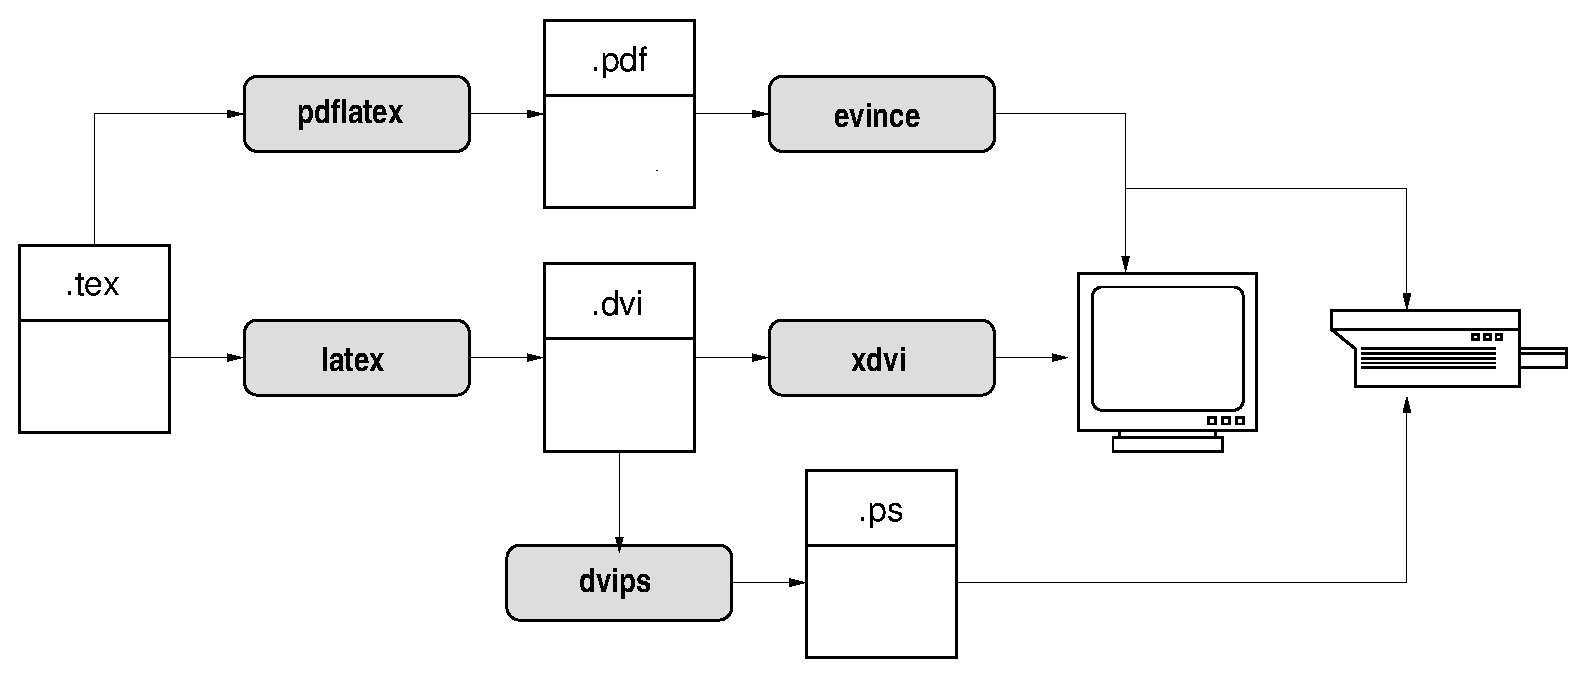
\includegraphics[width = 0.8\linewidth]{img/cycle.eps}
    \caption{UNIX中参与生成过程的工具}
    \label{fig:1.2}
\end{figure}

\subsection{显示}%visualisation有时翻译成可视化,有时翻译成显示,这个可以后期再统一一下。

在编译后,可以简单地使用\textsf{evince}程序来完成显示步骤。输入以下指令:

\dmh{evince \codereplace{文件名}.pdf \&}

这是一个\textsf{linux}下运行的十分直观的程序,能够给出一个方便阅读的文件预览。

\begin{exclamation}
    注意,不必在每次编译后都重新运行evince,它显示的内容会自动刷新。
\end{exclamation}

\subsection{打印}

对于\dm{pdf}格式,如何打印它这一问题就丢给了你的操作系统。关于这一点,没有特殊的注意事项。你有了一个文件,可以自由地处置它,无论是直接打印,还是根据你所处的环境来发挥才艺。

\begin{ii}
    从\dm{dvi}到\dm{ps}格式的转换需要调用dvips程序:

    \dmh{dvips \codereplace{文件名}.dvi}

    这可以生成一个PostScrpt格式的文件。这个格式也由Adobe创造,是一种打印机语言,可以看作\dm{pdf}的祖先。目前的打印机出厂即可识别这种打印机语言。我们可以说,文件发送到打印机时,十有八九传送的是PostScrpt格式的参数。对于PostScript格式的文件,有大量可以显示、修改这种文件的工具。
\end{ii}

\section{源文件的结构}

本节将介绍一种文档类型。实际上,所有\LaTeX 文档都具有相同的结构,形式如下:

\begin{dmd}
\backslash documentclass[\codereplace{类选项$_1$},\codereplace{类选项$_2$},...]\{\codereplace{类}\}\\
\backslash usepackage[\codereplace{包选项$_1$},\codereplace{包选项$_2$},...]\{\codereplace{包}\}\\
...\\
\codereplace{文前部分}\\
...\\
\backslash begin\{document\}\\
...\\
\codereplace{文本}\\
...\\
\backslash end\{document\}
\end{dmd}

如此一来,所有的\LaTeX 文档都可以按以下方式拆解。

\begin{itemize}
    \item 说明文档的\codereplace{类};
    \item 文前部分,包含以下内容:
        \begin{itemize}
            \item 使用特定的\codereplace{包};
            \item 多样的初始化和声明;
        \end{itemize}
    \item 文档主体,即我们将要亲手输入的全部内容,出现在\dm{\backslash begin\{document\}}和\dm{\backslash end\{document\}}之间。
\end{itemize}

以下介绍各部分的细节。

\subsection{文档的类}

所谓类,就是提供给\LaTeX 的一个指示,可以帮助\LaTeX 决定如何为文档的特定部分排版。根据具体使用的类不同,允许使用与否的指令可能不同(如\dm{\backslash chapter}在\dm{book}类中允许使用,在\dm{article}类中不允许使用)。另一方面,根据所选择的类,给出的命令会具有特定的含义(标题、材料表……)。在入门时\jz{
    实际上,我们可以在\dm{\backslash documentclass}前添加更多神奇的“咒语”……
},所有的\LaTeX 文档都必须以的指令开始——\dm{\backslash documentclass}接由花括号括住的类,包含以下几种:

\begin{itemize}
    \item \dm{article},用于文章;
    \item \dm{proc},用于电气与电子工程师协会(英:Institute of Electrical and Electronics Engineers,IEEE)会刊(英:proceeding)风格的文章;
    \item \dm{report},用于几十页篇幅的报告;
    \item \dm{book},用于图书或论文;
    \item \dm{letter},用于信件;
    \item \dm{slides},用于演示文档。
\end{itemize}

我们当然也可以为文档定义自己的类。类的配置项用方括号括住,可以是以下内容之一:

\begin{itemize}
    \item \dm{11pt, 12pt},用于全局地更改文字字号;
    \item \dm{twoside},用于生成适合双面打印的文档;
    \item \dm{draft},用于以草稿模式生成文档。
\end{itemize}

例如,输入:

\begin{dmd}
\verb|\documentclass{article}|
\end{dmd}

以上命令可以将全部配置项配置为默认值(字号为10 pt,单列,单面……)。

\begin{dmd}
    \backslash documentclass[12pt]\{article\}
\end{dmd}

以上命令将字号设置为12 pt(默认为10 pt)。再如:

\begin{dmd}
    \backslash documentclass[twoside, draft]\{report\}
\end{dmd}

以上命令可以以草稿模式生成适合双面打印的报告。

\subsection{文前部分}

文前部分是指位于子句\dm{\backslash documentclass}和子句\dm{\backslash begin\{documennt\}}间的区域。在这个区域中,我们可以明确想要包含的扩展(请看下一小节)%TODO
、初始化全局参数(如页边距等)、定义风格(如标题样式、序号等)、定义特殊的宏,等等。

\subsection{添加扩展}

\LaTeX 命令\dm{\backslash usepackage}可以与C语言的指令\dm{\#include}类比。这一命令允许添加\LaTeX 中满足宏或环境形式的功能\jz{
    相关内容将在下一章讲解。%TODO
}。目前,只需记住,我们可以在一行之内包含多个包:

\begin{dmd}
    \backslash usepackage\{\codereplace{包$_1$},\codereplace{包$_2$},\codereplace{包$_3$},...\}
\end{dmd}

如果\codereplace{包$_1$}、\codereplace{包$_2$}、\codereplace{包$_3$}拥有共同的配置项\codereplace{opt1},我们可以输入:

\begin{dmd}
    \backslash usepackage[\codereplace{opt1}]\{\codereplace{包$_1$},\codereplace{包$_2$},\codereplace{包$_3$}\}
\end{dmd}

相反,如果\codereplace{opt1}只涉及\codereplace{包$_2$},那么我们只能像这样写成两行:

\begin{dmd}
    \backslash usepackage\{\codereplace{包$_1$},\codereplace{包$_3$}\}\\
    \backslash usepackage[\codereplace{opt1}]\{\codereplace{包$_2$}\}
\end{dmd}

下面是两个例子:

\begin{dmd}
    \% 包graphicx带有配置项draft和xdvi\\
    \backslash usepackage[xdvi, draft]\{graphicx\}\\
    \% 包array和包subfig\\
    \backslash usepackage\{array, subfig\}
\end{dmd}

\begin{exclamation}
    根据定义,所有(类、包、命令的)的配置项参数都是\textit{可选的}。因此我们可以这样记:\LaTeX 中所有由方括号括住的参数\dm{[...]}都是非强制的。
\end{exclamation}

\section{开始!}

在本节,我们将尝试从一个只含几个排版命令的文档开始,介绍\LaTeX 的基本原理。

\begin{codelist}[1.1]{
    从你手中掉落的工具总是掉到最难够到的地方,或脆弱的物品上。\\
    这是\emph{墨菲}定律(loi de Murphy)的一个体现。
}  \begin{dmd}
    \verb+\documentclass{article}+\\
    \verb+\begin{document}+\\
    从你手中掉落的工具\\
    总是掉到最难够到的地方,\\
    或脆弱的物品上。\\
    ~\\
    \verb+这是\emph{墨菲}定律(loi de      Murphy)的+\\
    一个体现。\\
    \verb+\end{document}+
\end{dmd}
\end{codelist}

这个示例体现了\LaTeX 中的几个重要的原理,具体如下。

\paragraph*{空行代表跳转至下一段} \LaTeX 中的空行代表一段文字的结尾,因此在以上实例中,第一段从“\dm{从你}”开始,直到“\dm{物品上。}”结束。指令\dm{\backslash par}与空行等价,可以用来表示一段文字的起始。

\paragraph*{\LaTeX 会忽略换行}最终的文档中,换行并不由源文件中的换行决定。\LaTeX 会自动为各段文本\textit{打断、压缩、调节}文字,除非你有特殊的要求。

\paragraph*{\LaTeX 会忽略重复的空格}输入1个或18784个空格是等价的,比如源码中\dm{de}和\dm{Murphy}前插入的空格那样。此规则也适用于跳转段落:输入一行或多行空格是等价的。

\paragraph*{“\backslash ”是转义字符(caractère d’échappement;英:escape char)}“\backslash ”可以告诉\LaTeX 它后面的一系列字符是控制序列,也就是说,是最一般意义上的指令(或宏)。这里,它对“墨菲”一词生效,具体的效果由指令\dm{\backslash emph}控制。

\paragraph*{“\{”和“\}”}它们是\textit{组}的定界符,稍后会进一步解释它们。

\subsection{几个特殊字符}

就像符号“\backslash”的出现所暗示的那样,\LaTeX 中还有10个有特殊含义的符号,在此将其列出:

\begin{dmd}
    \verb+\ $ & % # ^ _ { } ~+
\end{dmd}

%todo 此前代码可以重新简化为verb

以下是一个使用部分特殊字符的案例:

\begin{codelist}[1.2]{
\textbf{是}下标:$x_{i+1}$,还是上标:$e^{i\pi}$;这是问题~1!
}\begin{verbatim}%毫无意义的段落
\textbf{是}下标:$x_{i+1}$,
还是上标:$e^{i\pi}$;
这是问题~1!%还是问题2?\end{verbatim}
\end{codelist}

目前,你需要知道:

\begin{itemize}
    \item \dm{\%}会使得\LaTeX 忽略当前行的剩余部分,因此,它是表示注释的符号(与C中的\dm{//}等价);
    \item \verb+~+代表不可拆分的空格\jz{
        见2.10节。
    },可以防止\LaTeX 在指定的位置断字。尽管有大量的情况需要插入这个符号来表示不可拆分(如所有形如“\verb+图~1+”的情况),然而,对于此类符号的使用,并没有系统化的规则。
    \item \dm{\$}用于标记公式的开始和结束。\LaTeX 遇到一个\dm{\$}符号时,它会切换到\celan{第3章}数学模式,直到遇到下一个\dm{\$}符号。
    \item \dm{\_}和\dm{\^{}}分别代表将文本转化为下标和上标。\textbf{注意},这两个符号只能在数学模式下使用。
    \item \dm{\{}和\dm{\}}分别表示组的开始和结束。本例中出现了两种组:一种出现在数学模式中,用于把将要放到下标或上标的“子公式”组合起来;另一种把将要设置成粗体的文字组合起来。
\end{itemize}

我们可以使用如下的指令来在让文档生成部分特殊字符:

\begin{dmd}
    \verb+\$ \& \% \# \{ \} \_+
\end{dmd}

这串指令可以输出“\$ \& \% \# \{ \} \_”。2.2.5小节%TODO
会解释如何使文档生成其余特殊字符(即\verb+\ ~ ^+)。

\subsection{调用指令}

你已经知道了,要想调用指令或宏,需要输入转义字符,并紧接着输入你想使用的宏名。%TODO 二对一
但是,\LaTeX 如何知道宏名的末尾在哪里呢?此处以用于生成\TeX 标识的\dm{\backslash TeX}为例来解释\yz{
    此例涉及对西文行文中空格的处理,不宜翻译。
}。

\begin{codelist}{
    \TeX book is for \TeX hackers.

    \TeX\  has some powerful macros.

    \LaTeX{} is a document preparation system
}\begin{verbatim}\TeX book is for \TeX hackers.

\TeX\  has some powerful macros.

\LaTeX{} is a document preparation system
    \end{verbatim}
\end{codelist}

\begin{exclamation}
    \verb*|\ |(其中\verb*| |代表空格)称作控制空格(espace de contrôle)。这个空格不会被\LaTeX 忽略。因此,指令“\verb*|et\ \ \ hop !|”会生成“et\ \ \ hop !”。实际上,以\dm{\backslash}\codereplace{函数}\dm{\{}\codereplace{参数}\dm{\}}的形式来调用宏是很好的习惯。因此,使用上例中的的第三种方式比第二种方式更佳。这种形式可以避免空格被忽略的情况发生\jz{
        所以他为什么要跟我们说这些?!
    }。因此,我们将使用\verb|the \teX{}book|来生成“the \TeX{}book”,使用“\verb*|\LaTeX{} is a ...|”来生成“\LaTeX{} is a ...”。
\end{exclamation}

\subsection{变音符号}

法国人往往对于使用\LaTeX 这件事忧心忡忡,因为法文中带有变音符号。别怕!你不必像表\ref{tab:1.1}\yz{
    该表与原书不完全相同。
}中展示的那样输入带有变音符号的字符。然而,你需要知道:无论是什么种类的字符,包括大写字母,我们都可以为其添加变音符号。

\begin{table}[H]
    \centering
    \begin{tabular}{|c|c|c|}
        \hline
        变音符号 & 源码 & 效果\\
        \hline
        尖音符 & \verb|\`z| & \`z \\
        钝音符 & \verb|\'z| & \'z \\
        长音符 & \verb|\^z| & \^z \\
        软音符 & \verb|\c{z}| & \c{z}\\
        分音符 & \verb|\"{z}| & \"{z}\\
        \hline
    \end{tabular}
    \caption{输入占7位(bit)的变音符号}
    \label{tab:1.1}
\end{table}

注意!虽然我们可以输入带有变音符号的字符,但不要忘记:这需要我们调用编码。目前,编码可能只针对地球上的某个地区。在法国,我们使用ISO 8859编码,配合拉丁文1区拓展。这套编码允许我们操纵美丽的变音符号。在详细阅读本书中专为使用法文书写文档的情况准备的章节\celan{第7章}之前,我们建议你在你源码的文前部分添加以下指令,以“攻克”法文文档的难关:

\begin{dmd}
    \begin{verbatim}
%源文件编码
\usepackage[latin1]{inputenc}
%TeX字体编码
\usepackage[T1]{fontenc}
%针对法文文档
\usepackage[francais]{babel}
    \end{verbatim}
\end{dmd}

\section{第一批工具}

以下几个宏和合字在文档中很常用,因此应当了解它们。首先,\LaTeX 会区分三种连接号:

\begin{itemize}
    \item \verb|-|,用于“Saint-Étienne”;
    \item \verb|--|,用于“page 12--24”;
    \item \verb|---|,在法文中用于插入语,如“une parenthèse --- comme cela”。
\end{itemize}

引号应以如下方式输入:

\begin{itemize}
    \item \verb|``|和\verb|''|可以输入英文中的引号\yz{
        此处与原书不同。原书前文输入变音符号时亦直接使用了单弯引号‘和’,但这两个符号作为命令参数时会导致编译错误,因此分别替换为反引号和直单引号。这可能是编译器的差异导致的。
    }——``English''。
    \item 如果键盘允许,对于法文,你可以输入«和»\jz{
        例如,在Linux系统下,分别按键盘的\fbox{Alt Gr}+\fbox{Z}和\fbox{Alt Gr}+\fbox{X}组合键(译注:适用于AZERTY键盘)。
    }。\textsf{babel}包的法文支持部分(参考第7章)%TODO
    允许我们通过\verb|\og|和\verb|fg|输入引号,由此,\verb|\og français\fg{}|这类命令是允许的—— «~français~»~。
\end{itemize}

以下是其余几个使用的命令:

\begin{itemize}
    \item \verb|\today|可以生成(编译时的)日期——2013年11月22日。
    \item \verb|\S|可以生成段落符号——\S。
    \item \verb|\ldots|可以在英文文档中生成省略号“\ldots”。但在法文文档中,应当输入三个点“...”(第7章会介绍更多有关法文排版的内容)。%TODO
\end{itemize}

最后要记得,英文中的双成分标点(ponctuation double;包括:;!?)前不加空格,但法文相反,它们的前面需要加空格。另外,在法国这个可爱的国家,我们几乎都靠右行驶。

\section{第一组报错}

\begin{ii}
    接下来,我们会看看\LaTeX 编译你的文档时闹的“情绪”。当我们放出编译指令时,我们会直接在终端看到这些输出。为了能让\LaTeX 得到充分使用,我们鼓励你在自己的环境下找到属于你自己的检查\LaTeX “\textsf{日志}”的方法。这些日体可以为你指明错误信息,以及编译过程中出现的其他警告。
\end{ii}

\subsection{症状}

如果你与\LaTeX 打交道,那么早晚有一天,你会看到屏幕上显示出类似这样粗旷的信息:

\begin{dmd}
    \linenumbers
    \begin{verbatim}
This is TeX, Version 3.1415 (C version 6.1)
(erreur.tex
LaTeX2e <1995/12/01>
(/usr/local/lib/texmf/tex/cls/article.cls
Document Class: article 1995/11/30 v1.3p Standard LaTeX document class
(/usr/local/lib/texmf/tex/clo/size10.clo)) (erreur.aux)
! Undefined control sequence.
l.5 paragraphe de ce \empha
                           {document}
?\end{verbatim}
\end{dmd}

几乎可以肯定,你看不懂这团内容。它是使用\LaTeX 处理文件\dm{erreur.tex}后终端上显示的内容。以下是文件全文\yz{
    文件正文意为:\dm{我觉得,在这样短的\backslash empha\{文档\}的第一段就有一个错误}。
}:

\begin{dmd}
    \begin{verbatim}
\documentclass{article}

\begin{document}
Il me semble bien qu’il y ait une erreur dans le
premier paragraphe de ce \empha{document} somme
toute assez court.
\end{document}
    \end{verbatim}
\end{dmd}

\subsection{诊断}

我们可以以一种简单的方式来解释以上错误信息。

\paragraph*{第1行}你使用的\TeX 版本为$\pi\pm 10^{-4}$。
\paragraph*{第2行}你想编译文件\dm{erreur.tex}。
\paragraph*{第3行}你使用了\LaTeXe ,版本日期为1995年12月。
\paragraph*{第4行~第5行}你使用了标准文档类\dm{article}。
\paragraph*{第6行}字号默认设置为10 pt。
\paragraph*{第7行}错误信息本身。
\paragraph*{第8行~第9行}\dm{erreur.tex}中造成错误的代码行和对应行号。
\paragraph*{第10行}\TeX 给出的短促且尤其让人焦虑的消息:\dm{?}。

第8行和第9行之间的“裂缝”精准地表明了\LaTeX 崩不住了的地方。以下消息:

\begin{dmd}
    ! Undefined control sequence.
\end{dmd}

向你说明了,\LaTeX 不认识你输入的指令。实际上,指令\verb|\empha|不存在。

\subsection*{治疗方案}

那么,当\LaTeX 给我们展示这个著名的“\dm{?}”时,我们应该怎么回答它呢?这里有3种最简短的方式,可以用来与\LaTeX 轻度交流。

\begin{itemize}
    \item 按回车键来忽略错误。
    \item 输入\dm{x}来退出编译。
    \item 输入\dm{r}让\LaTeX 继续编译,并忽略其他错误信息。
    \item 输入\dm{i}以插入一条更正信息并继续编译,但新插入的更正信息并不会出现在源文档中。
    \item 输入\dm{h}以获取更多关于该错误的信息。以下是本例中\TeX 提供给你的更多信息:\begin{verbatim}
Undefined control sequence :
  The control sequence at the end of the top line
  of your error message was never \def’ed. If you have
  misspelled it (e.g., ‘\hobx’), type ‘I’ and the
  correct spelling (e.g., ‘I\hbox’). Otherwise just
  continue, and I’ll forget about whatever was
  undefined.\end{verbatim}
\end{itemize}

\subsection{一些消息}

\TeX 和\LaTeX 会根据不同的情况给出大量错误消息,其中有一些在第一次面对时并不能读懂。然而,大多数经常出现的消息有以下类型:

\begin{itemize}
    \item \LaTeX 语法或保留字错误;
    \item 花括号没有成对出现;
    \item 在文本模式中出现了本应出现在数学模式中的内容;
    \item 数学模式没有关闭;
    \item 你忘记包含一个包;
    \item 编译过程无法结束;%TODO核实
    \item ……
\end{itemize}

\section{再说几句!}

现在,你知道了如何用\LaTeX 源码创建可打印的文件。同时,本章向你介绍了调用指令的原则。接下来,如果想要了解\LaTeX 语法中的不同功能,需要做的仅仅是去着手接下来的章节。%TODO
% \begin{appendices}
%     \section{附录}
% \end{appendices}
\end{document}